\documentclass{article}
\usepackage{listings}
\usepackage{color}
\usepackage{amsmath}
\usepackage{graphicx}
\usepackage{float}
\usepackage[linguistics]{forest}
\usepackage[utf8]{inputenc} 
\usepackage{chngcntr}
\counterwithin*{section}{part}
\definecolor{mGreen}{rgb}{0,0.6,0}
\definecolor{mGray}{rgb}{0.5,0.5,0.5}
\definecolor{mPurple}{rgb}{0.58,0,0.82}
\definecolor{backgroundColour}{rgb}{0.95,0.95,0.92}
\lstdefinestyle{CStyle}{
    backgroundcolor=\color{backgroundColour},   
    commentstyle=\color{mGreen},
    keywordstyle=\color{magenta},
    numberstyle=\tiny\color{mGray},
    stringstyle=\color{mPurple},
    basicstyle=\footnotesize,
    breakatwhitespace=false,         
    breaklines=true,                 
    captionpos=b,                    
    keepspaces=true,                 
    numbers=left,                    
    numbersep=5pt,                  
    showspaces=false,                
    showstringspaces=false,
    showtabs=false,                  
    tabsize=2,
    language=C
}

\title{PLDAC}
\author{Buton Nicolas}
\renewcommand{\contentsname}{Table des matières}
\begin{document}
\pagenumbering{gobble}
\maketitle

\includegraphics[scale=1]{images/logoSorbonne.jpg}
\newpage
\tableofcontents
\newpage
\pagenumbering{arabic}
\part{Intro}
\section{Decription du dataset}
Fréquence d'échantillonage : 512Hz\\
Nombre de participant : 20 (7 femmes, 13 hommes)\\
Age : \\
mean: 25.8 \\
sd : 5.27 \\
median 25.5\\
18 subjects between 19 and 28 years old.\\
Two participants with age 33 and 44 were outside this range.\\
Nombre d'éléctrode : 16\\
\begin{figure}[H]
\begin{center}
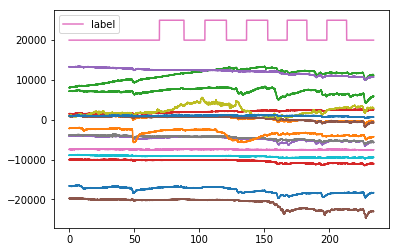
\includegraphics[scale=0.8]{images/donnees_entree.png}
\end{center}
\caption{Affichage des données brut}
\end{figure}

\section{Les diférentes méthodes}
\begin{forest}
[Brut
  [Filtre passe-bas
	[Percetron(8)]  
	[KNN(9)]
  ]
  [TF
  	[Percetron(1)]
  	[KNN(2)]
  ]
  [Cov
  	[Perceptron(3)]
  	[MDM(4)]
  	[KNN(5)]
  ]
  [Perceptron(6)]
  [KNN(7)]
]
\end{forest}
Légende :\\
Cov : Matrice de covariance\\
TF : Transformé de fourier\\
MDM : Minimum Distance to Mean\\
\\
Prédiction théorique : \\
La méthode 6 et 7 ne devrais pas fonctioner car avec une seule données c'est difficile de faire quoi que ce soit.\\
La méthode 8 et 9 ne devrais pas fonctionner car il n'y aura pas invariance par translation et on ne pourra pas connaitre le debut.
\part{Résultat des différents algorithmes}
\section{Perceptron sur les données brut}
\begin{figure}[H]
\begin{center}
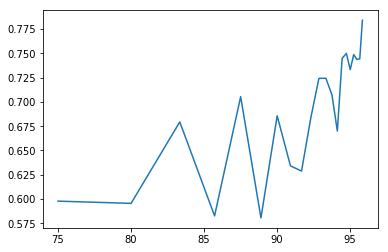
\includegraphics[scale=1]{images/perceptron_brut_f1Score.png}
\end{center}
\caption{F1 score(en cross validation) du perceptron en fonction du pourcentage des données utilisé pour le train}
\end{figure}
$
clf = SGDClassifier(loss="perceptron", eta0=1e-4, learning_rate="constant", penalty=None,tol=1e-1,max_iter=10000,shuffle=True)
$
\section{KNN sur les données brut}
\begin{figure}[H]
\begin{center}
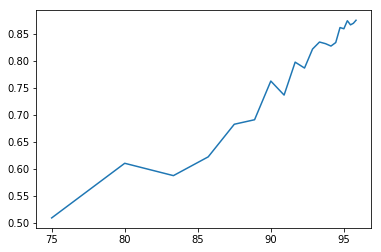
\includegraphics[scale=1]{images/knn_brut_f1Score.png}
\end{center}
\caption{F1 Score(en cross validation) du knn en fonction du pourcentage des données utilisé pour le train}
\end{figure}
$
neigh = KNeighborsClassifier(n_neighbors=10)
$
\section{Riemann Cov MDM }
\begin{figure}[H]
\begin{center}
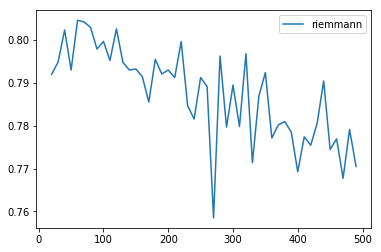
\includegraphics[scale=1]{images/riemann_cov_MDM_f1Score.png}
\end{center}
\caption{F1 Score(en cross validation) de riemann MDM en fonction du nombre de données par paquet}
\end{figure}

estimer la matrice de covariance\\
$
cov = pyriemann.estimation.Covariances().fit_transform(X)
$
\\
validation croisée\\
$
mdm = pyriemann.classification.MDM()
$
\section{Riemann Cov KNN }
\begin{figure}[H]
\begin{center}
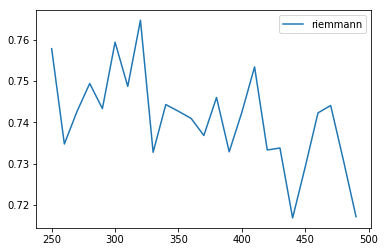
\includegraphics[scale=1]{images/riemann_cov_knn_f1Score.png}
\end{center}
\caption{F1 Score(en cross validation) du riemann knn en fonction du nombre de données par paquet}
\end{figure}

estimer la matrice de covariance\\
$
cov = pyriemann.estimation.Covariances().fit_transform(X)
$
\\
validation croisée\\
$
knn = pyriemann.classification.KNearestNeighbor(n_neighbors=10)
$
\section{Perceptron filtre passe bas }
\begin{figure}[H]
\begin{center}
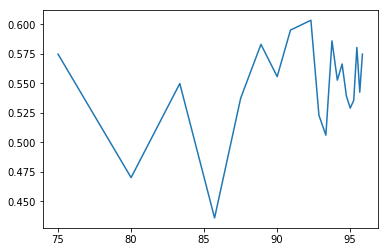
\includegraphics[scale=1]{images/perceptron_passe_bas_f1Score.png}
\end{center}
\caption{F1 Score(en cross validation) du perceptron en fonction du pourcentage des données utilisé pour le train}
\end{figure}
\\
$
 clf = SGDClassifier(loss="perceptron", eta0=1e-4, learning_rate="constant", penalty=None,tol=1e-1,max_iter=10000,shuffle=True)
    
$

\section{KNN filtre passe bas }
\begin{figure}[H]
\begin{center}
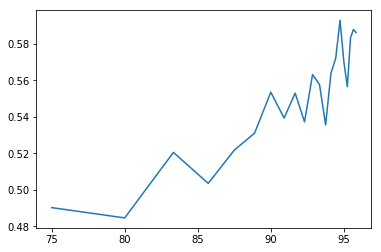
\includegraphics[scale=1]{images/knn_passe_bas_f1Score.png}
\end{center}
\caption{F1 Score(en cross validation) du knn en fonction du pourcentage des données utilisé pour le train}
\end{figure}

estimer la matrice de covariance\\
$
neigh = KNeighborsClassifier(n_neighbors=10)
    y_pred = cross_val_predict(neigh,donnees,labels,cv=k)
$
\\


\section{Perceptron transformée de fourier }
\begin{figure}[H]
\begin{center}
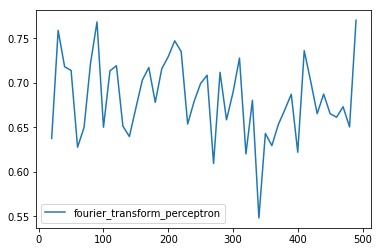
\includegraphics[scale=1]{images/perceptron_tf_f1Score.png}
\end{center}
\caption{F1 Score(en cross validation) du perceptron en fonction}
\end{figure}

estimer la matrice de covariance\\
$
cov = pyriemann.estimation.Covariances().fit_transform(X)
$
\\
validation croisée\\
$
knn = pyriemann.classification.KNearestNeighbor(n_neighbors=10)
$
\section{KNN transformée de fourier }
\begin{figure}[H]
\begin{center}
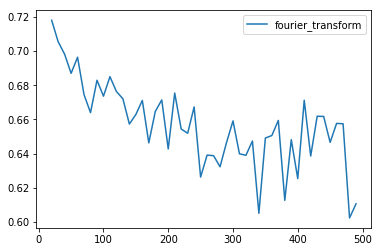
\includegraphics[scale=1]{images/knn_tf_f1Score.png}
\end{center}
\caption{F1 Score(en cross validation) du knn en fonction}
\end{figure}

estimer la matrice de covariance\\
$
cov = pyriemann.estimation.Covariances().fit_transform(X)
$
\\
validation croisée\\
$
knn = pyriemann.classification.KNearestNeighbor(n_neighbors=10)
$
\end{document}
